\chapter{Applicazione realizzata}
Il progetto di tesi proposto ha come focus principale la realizzazione del docking tra i ligandi contenuti in specifici pesticidi e i recettori dell'apis mellifera e l'estrazione dei legami che si vengono a formare. 

\section{Installazione}
L'applicazione viene scaricata dalla \href{https://github.com/mungowz/Computational-Docking.git}{repository di github} mediante il comando:

\begin{lstlisting}[language=Bash, label=lst:code1, caption={Comando per scaricare la repository}]
git clone https://github.com/mungowz/Computational-Docking.git
\end{lstlisting}

Verrà quindi installata nella directory corrente la repository contenente il progetto, all'interno di questa si trovano gli script utilizzati dall'applicazione e le directory ed i file di input di default, tra cui:

\begin{itemize}
    \item Il file di input dei ligandi, ovvero \textit{ligands\_list.txt}
    \item La directory contenente la lista di default dei ligandi, ovvero \textit{/data/files/}
    \item La directory di default che conterrà i file \textit{.xlsx} di output prodotti, ovvero \textit{/output/excel\_files}
    \item La directory di default che conterrà i file \textit{.sdf} prodotti, ovvero \textit{/data/ligands/sdf/}
    \item Le directory di default che conterranno i file \textit{.pdb} prodotti, ovvero \textit{/data/ligands/pdb/} per i ligandi e \textit{/data/proteins/pdb/} per i recettori
    \item Le directory di default che conterranno i file \textit{.pdbqt prodotti}, ovvero \textit{/data/ligands/pdbqt/} per i ligandi e \textit{/data/proteins/pdbqt/} per i recettori.
\end{itemize}

Sarà necessario inoltre installare alcune dipendenze esterne (software esterni) ed interne (librerie e pacchetti di python) per far funzionare l'applicazione, la lista delle dipendenze e la procedura di installazione è specificata nel file \textit{README} della repository di github.

\section{Modalità di utilizzo}
Il software realizzato può essere utilizzato in due modalità: mediante script python da terminale o mediante interfaccia grafica realizzata seguendo il paradigma \textit{model-view-controller}.\newline
Non sarà necessario effettuare ulteriori installazione per usufruire di entrambe le modalità ma bisognerà semplicemente scaricare la repository e seguire le istruzioni del \textit{README}.\newline
Per eseguire l'applicazione da riga di comando devono essere eseguiti separatamente nell'ordine i seguenti script:
\begin{itemize}
    \item \textbf{prepare\_ligands.py}
    \item \textbf{prepare\_receptors.py}
    \item \textbf{performDocking.sh}
\end{itemize}

La GUI usufruirà degli stessi lanciati da riga di comando il che garantisce le stesse funzionalità in entrambe le modalità di utilizzo e seguendo i dettami della \textbf{OOP} secondo i quali bisogna riutilizzare codice funzionante anzichè modificarlo o scriverne di nuovo.\newline
Per avviare la GUI deve essere digitato nel terminale il comando:

\begin{lstlisting}[language=bash, label=lst:code2, caption={Comando per avviare la GUI}]
python app.py    
\end{lstlisting}

Avviando la GUI si aprirà la home page con le seguenti opzioni:

\begin{itemize}
    \item Opzione \textbf{Preparation}: si accede alla sezione relativa alla preparazione degli input
    \item Opzione \textbf{Docking}: sarà possibile effettuare il docking
    \item Opzione \textbf{Analysis}: sarà possibile effettuare l'analisi dei risultati del docking
    \item Opzione \textbf{Help}: si accede alla sezione relativa alle informazioni utili per l'utente per l'uso del software.
\end{itemize}

\begin{figure}[H]
    \centering
    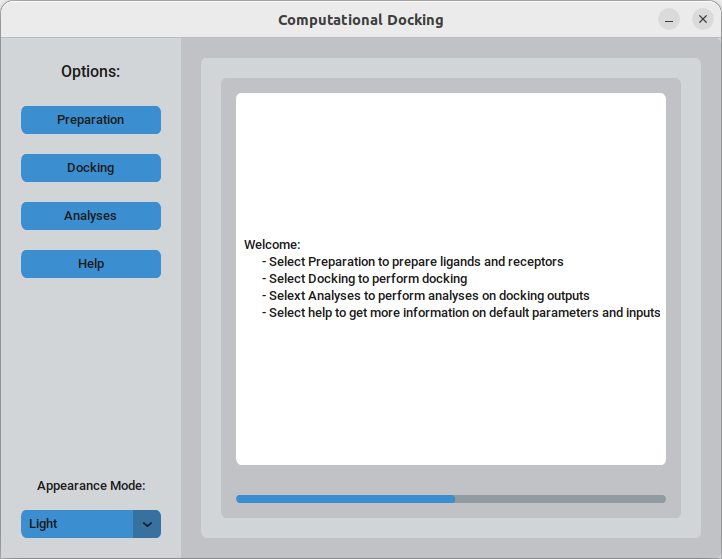
\includegraphics[scale=0.6]{immagini/homePage.png}
    \caption{Sezione \textbf{Home Page} della GUI}
    \label{fig:Home Page}
\end{figure}

\section{Dati in input}
I dati in input all'applicazione trattata sono: ligandi e proteine. La lista dei ligandi è fornita in input tramite foglio calcolo (\textit{.xlsx}, \textit{.xls}) o mediante file di testo (\textit{.txt}), 
in entrambi i casi ogni riga corrisponde al nome di un ligando. Essendo l'applicazione incentrata sullo studio degli effetti dei ligandi dei pesticidi sull'apis mellifera, 
come dati di esempio sono state utilizzati i ligandi le cui molecole costituiscono i pesticidi maggiormente diffusi sul mercato, per un totale di 297 ligandi. La lista è disponibile nell'appendice \ref{tab:Tabella dei Ligandi}.\newline
I recettori vengono selezionati mediante una \textbf{web view} aperta sulla pagina di ricerca del sito di \href{https://www.rcsb.org/search}{PubChem}, quivi l'utente digiterà la propria query e 
dopo aver selezionato il  tasto \textbf{research} gli verranno mostrati tutti i composti organici relativi alla query digitata, tramite il tasto \textbf{Get Query} l'utente andrà a 
scaricare tutti i file  dei composti organici in formato \textit{.pdb}. Nel caso di esempio sono state scelte tutte le proteine dei recettori dell'Apis Mellifera come mostrato nelle foto: 
\ref{fig:queryRecettori} e  \ref{fig:fileRecettori}, per un totale di 60 file \textit{.pdb} contenenti le strutture di determinate proteine. La lista delle proteine scaricate è disponibile nell'appendice: \ref{Tabella dei Recettori}. L'applicazione usata tramite GUI dispone della sezione \textbf{Help} (\ref{fig:help}) contenente le informazioni relative alle impostazioni di default e al formato dei dati in input.

\begin{figure}[H]
    \centering
    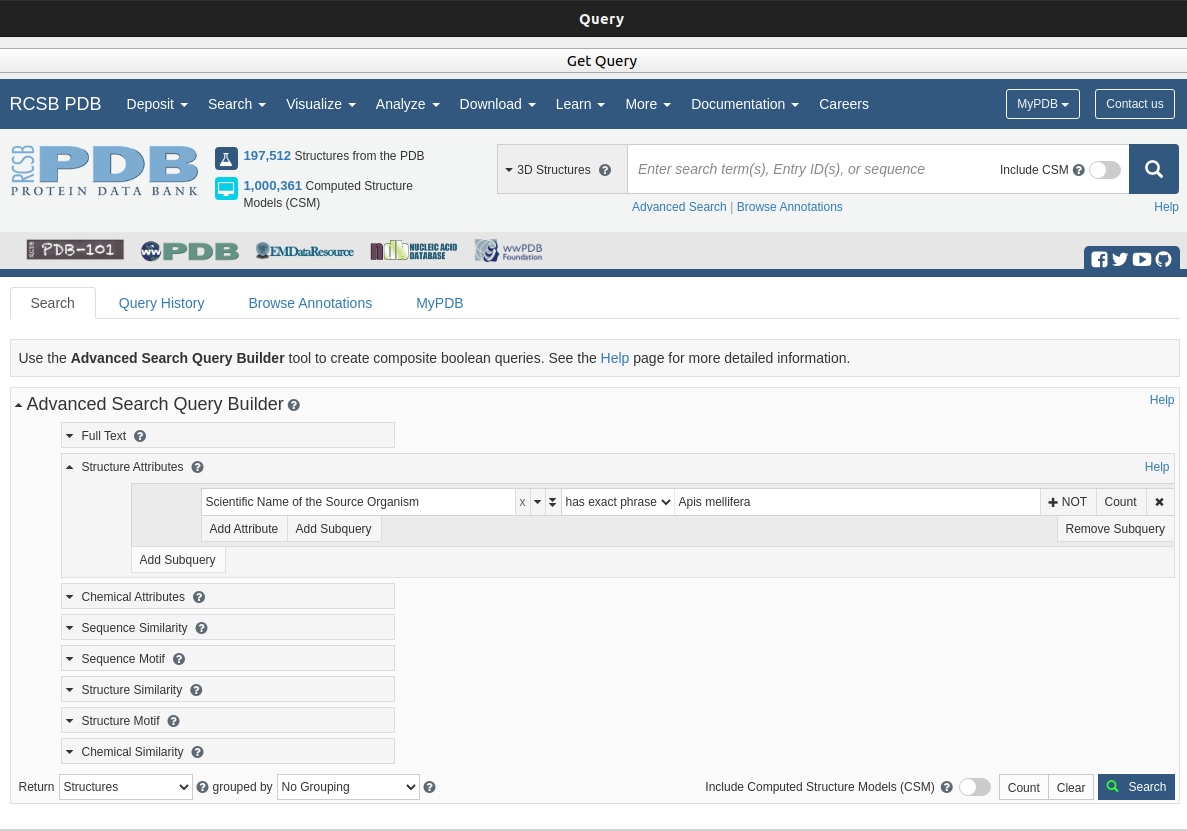
\includegraphics[scale=0.4]{immagini/queryRecettori.png}
    \caption{Query dei recettori}
    \label{fig:queryRecettori}
\end{figure}

\begin{figure}[H]
    \centering
    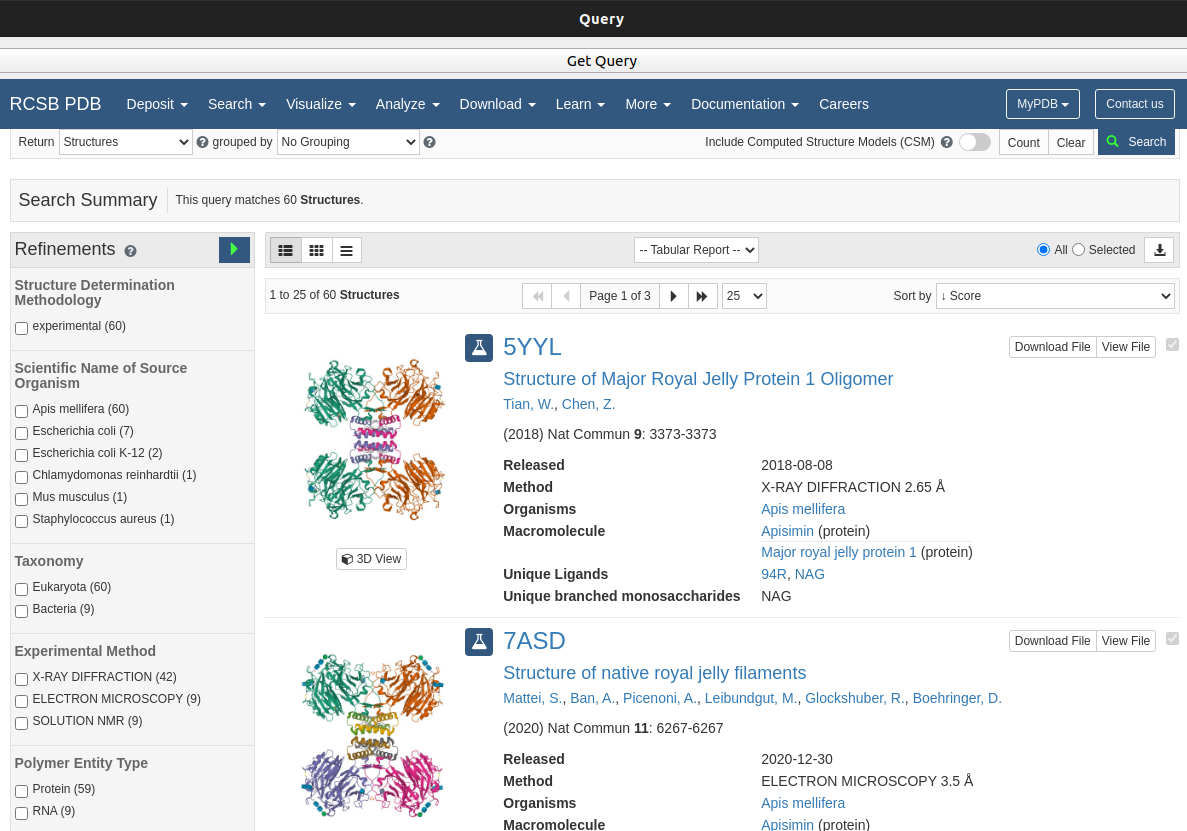
\includegraphics[scale=0.4]{immagini/fileRecettori.png}
    \caption{Proteine dei recettori dell'apis mellifera}
    \label{fig:fileRecettori}
\end{figure}

\begin{figure}[H]
    \centering
    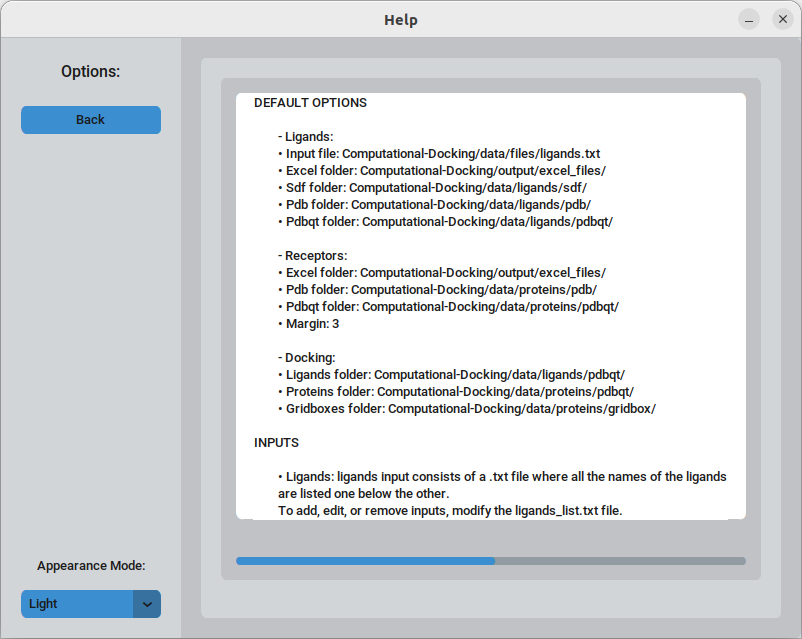
\includegraphics[scale=0.6]{immagini/help.png}
    \caption{Sezione \textbf{Help} della GUI}
    \label{fig:help}
\end{figure}

\section{Preparazione dei ligandi e dei recettori}
Il primo step propedeutico per il docking è la preparazione dei ligandi e dei recettori, questa
fase viene esplicitamente eseguita dal software realizzato. L'intera fase è svolta: per i ligandi dallo script python \textbf{prepare\_ligands.py} mentre, per i recettori dallo script python \textbf{prepare\_receptors.py}. Se l'applicazione viene utilizzata mediante GUI la preparazione dei ligandi e dei recettori può essere effettuata mediante la sezione \textbf{Preparation} della pagina principale come mostrato in figura \ref{fig:preparation}.

\begin{itemize}
    \item Selezionando l'opzione \textbf{Ligands} si accede alla sezione relativa alla preparazione dei ligandi
    \item Selezionando l'opzione \textbf{Receptors} si accede alla sezione relativa alla preparazione dei recettori
    \item Selezionando l'opzione \textbf{Back} si ritorna alla pagina principale.
\end{itemize}


\begin{figure}[H]
    \centering
    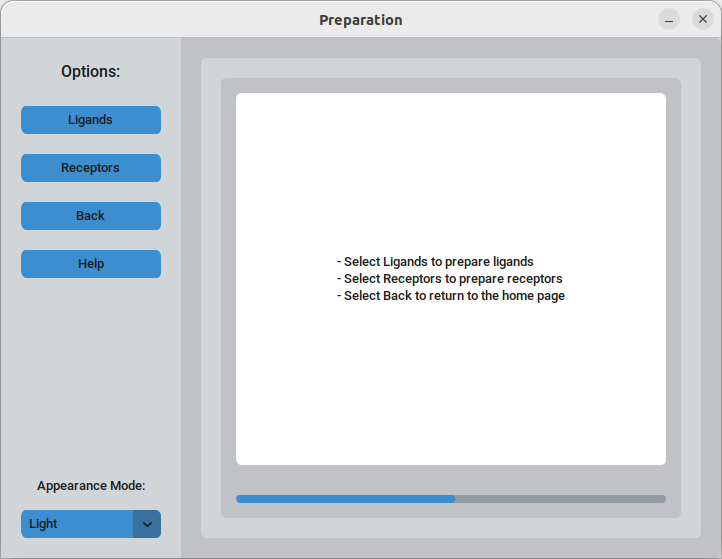
\includegraphics[scale=0.6]{immagini/preparation.png}
    \caption{Sezione \textbf{Preparation} della GUI}
    \label{fig:preparation}
\end{figure}

\subsection{Preparazione dei ligandi tramite script} \label{Preparazione dei ligandi script}
Lo script python \textbf{prepare\_ligands.py}, che esegue tale fase, viene eseguito da terminale mediante il comando:

\begin{lstlisting}[language=Bash, label=lst:code3, caption={Comando per scaricare la repository}]
python prepare_ligands.py
\end{lstlisting}

Questo script può ricevere diversi argomenti in input:

\begin{itemize}
    \item $[-v] | [--verbose]$: serve per attivare il verbose e se non viene specificata tale opzione viene lasciata di default inattivo
    \item $[-e] | [--input-file]$: specifica un nuovo file di input (\textit{.xlsx}, \textit{.xls}) o (\textit{.txt}) da cui prendere i nomi dei ligandi, se non viene specificata tale opzione verrà scelto il file di default scaricato insieme al software
    \item $[-E] | [--excel-folder]$: specifica la directory dei file \textit{.xlsx} di output, se non viene specificata tale opzione verrà scelta la directory di default
    \item $[-s] | [--sdf-folder]$: specifica la directory dei file \textit{.sdf} di output, se non viene specificata tale opzione verrà scelta la directory di default
    \item $[-P] | [--pdb-folder]$: specifica la directory dei file \textit{.pdb} di output, se non viene specificata tale opzione verrà scelta la directory di default
    \item $[-p] | [--pdbqt-folder]$: specifica la directory dei file \textit{.pdbqt} di output, se non viene specificata tale opzione verrà scelta la directory di default
    \item $[-k] | [--keep-ligands]$: specificando questa opzione viene scelto di non cancellare i file dei ligandi precedentemente scaricati, se non viene specificata tale opzione i file verranno cancellati
    \item $[-h] | [--help]$: stampa la spiegazione degli input per lo script.
\end{itemize}

Lo script quando eseguito andrà ad inizializzare i vari percorsi, e nel caso siano stati inseriti in input verrà controllata l'esistenza e la validità degli stessi. Nel caso non siano presenti le directory contenenti i file \textit{.sdf}, \textit{.pdb} e .\textit{pdbqt}, queste verranno create automaticamente dall'applicazione a meno di input inseriti dall'utente e saranno cancellati i file precedentemente scaricati a meno di input contrario.\newline
Lo script richiama la funzione \textbf{selectLigands} la quale si occupa di scaricare da \textbf{Pubchem}
i file \textit{.sdf} corrispondenti alla lista dei ligandi in input. La funzione prende in input: 

\begin{itemize}
    \item \textit{input\_path}, il path del file di input
    \item \textit{sdf\_folder}, il path della directory di output per i file \textit{.sdf}
    \item \textit{excel\_folder}, il path della directory di output per i file \textit{.xlsx}
    \item \textit{verbose}, il flag relativo al verbose.
\end{itemize}

In output ci vengono dati i file \textit{.sdf} corrispondenti ai ligandi in input, dove il nome di ogni file è preceduto dal suffisso \textit{ligand\_}, e un file \textit{.xlsx} contenente i risultati dell'operazione di download nominato \textit{ligands\_sdf\_output.xls}.

\begin{lstlisting}[language=Python, label=lst:code4, caption={funzione selectLigands}]
selectLigands(input_path, sdf_folder, excel_folder, verbose)
\end{lstlisting}

L'interfaccia con il database avviene tramite il pacchetto \textbf{PubChemPy}, in particolare la funzione \textbf{pubchempy.get\_compounds} permette di ricercare nel database il record relativo allo specifico ligando il cui nome, a cui viene precedentemente aggiunto il suffisso \textit{ligand\_}, gli viene fornito in input. Questa prende in input:

\begin{itemize}
    \item \textit{identifier}, il composto da ricercare nel database
    \item \textit{namespace}, il parametro in base al quale ricercare il composto, nel nostro caso il parametro scelto è il nome indicato dalla stringa \textit{"name"}
    \item \textit{record\_type} ovvero il tipo di record relativo al composto in questione da scaricare, 
    nel nostro caso il parametro scelto è la stringa \textit{"3d"} che indica la struttura 3D del ligando.
\end{itemize}

In output verrà fornito il record della struttura 3D del ligando in questione.

\begin{lstlisting}[language=Python, label=lst:code5, caption={funzione pubchempy.get\_compounds}]
pubchempy.get_compounds(identifier, "name", record_type="3d")
\end{lstlisting}

La funzione che effettivamente si occupa di scaricare la struttura 3D del ligando in formato \textit{.sdf}, richiamata da \textbf{selectLigands} è \textbf{pubchempy.download}, prende in input:

\begin{itemize}
    \item \textit{outformat}, il formato in cui deve essere scaricato il file,  nel nostro caso il parametro scelto è il formato \textit{.sdf} indicato dalla stringa \textit{"SDF"}
    \item \textit{path}, il path della directory in cui vengono scaricati i file \textit{.sdf}
    \item \textit{identifier}, il composto da scaricare nel database
    \item \textit{namespace}, il parametro in base al quale ricercare il composto, nel nostro caso il parametro scelto è il nome indicato dalla stringa \textit{"name"}
    \item \textit{record\_type} ovvero il tipo di record relativo al composto in questione da scaricare, 
    nel nostro caso il parametro scelto è la stringa \textit{"3d"} che indica la struttura 3D del ligando.
\end{itemize}

L'output di tale funzione sarà il file \textit{.sdf} del ligando in questione.

\begin{lstlisting}[language=Python,  label=lst:code6, caption={pubchempy.download}]
pubchempy.download("SDF", path, identifier, "name", record_type="3d")
\end{lstlisting}

I nomi di alcuni file potrebbero non essere presenti nel database oppure, a causa di spazi presenti nel loro nome, non essere riconosciuti. Nel primo caso i ligandi vengono semplicemente scartati nel secondo caso gli spazi vengono sostituiti da underscore (\_), seguendo quindi la nomenclatura del database, e viene effettuata nuovamente la ricerca di questi nel database. Se ancora la ricerca non ha successo il ligando in questione viene definitivamente scartato.\newline
Oltre ai file \textit{.sdf} la \textbf{selectLigands} produrrà anche un file \textit{.xlsx} contenente il riepigolo dei risultati ottenuti dalla funzione, ovvero:

\begin{itemize}
    \item file scaricati
    \item file scaricati con il nome modificato 
    \item ligandi non trovati all'interno del database.
\end{itemize}

Nel caso di esempio, dei 297 ligandi in input, 289 sono stati trovati e scaricati con successo, i restanti 8 sono stati scartati: \ref{tab:Ligandi scartati}.

\begin{table}[H]
    \centering
    \begin{tabular}{|l|l|}
    \hline
    Sodium 4-nitrophenolate & Silthiofa \\ \hline
    Sodium 2-methoxy-5-nitrophenolate & Potassium bicarbonate \\ \hline
    (E,E)-7,9-Dodecadien-1-yl acetate & Dodine \\ \hline
    Sodium 2-nitrophenolate & Ziram \\ \hline
    \end{tabular}
    \caption{Ligandi non scaricati}
    \label{tab:Ligandi scartati}
\end{table}

Dopo aver scaricato i file \textit{.sdf} questi devono essere convertiti in formato \textit{.pdb}, per fare ciò lo script richiama la funzione \textbf{sdf2pdb}, la quale prende in input:

\begin{itemize}
    \item \textit{sdf\_folder}, la directory con i file \textit{.sdf} in input
    \item \textit{pdb\_folder}, la directory con i file \textit{.pdb} in output
    \item \textit{verbose}, il flag relativo al verbose.
\end{itemize}

La funzione restituisce in output i file \textit{.pdb} corrispondenti a tutti i file \textit{.sdf} dati in input.

\begin{lstlisting}[language=Python, label=lst:code7, caption={funzione sdf2pdb}]
sdf2pdb(sdf_folder, pdb_folder, verbose)
\end{lstlisting}

La funzione usufruisce del programma \textbf{Open babel} in particolare esegue la conversione da \textit{.sdf} a \textit{.pdb} richiamando la sua versione da terminale tramite il comando \textbf{obabel}:

\begin{lstlisting}[language=Bash, label=lst:code8, caption={Comando per la conversione da \textit{.sdf} a \textit{.pdb}}]
obabel sdf_file_path -O pdb_path
\end{lstlisting}

Nell'istruzione sopra \textit{sdf\_file\_path} indica la directory con i file \textit{.sdf} in input, la directory con i file \textit{.pdb} in output, \textit{pdb\_path}, viene specificata tramite lo switch \textit{-O}. Tramite tale istruzione è possibile effettuare la conversione di un singolo file, la conversione di tutti i \textit{.sdf} avviene ciclando su tutti i file nella directory corrispondente.\newline
L'ultimo step nella preparazione dei ligandi è effettuato dalla funzione \textbf{prepareLigands}, questa funzione prende in input:

\begin{itemize}
    \item \textit{pdb\_folder}, la directory con i file \textit{.pdb} in input
    \item \textit{pdbqt\_folder}, la directory con i file \textit{.pdbqt} in output
    \item \textit{verbose}, il flag relativo al verbose.
\end{itemize}

La funzione restituisce la conversione in file \textit{.pdbqt} dei corrispondenti i file \textit{.pdb} dati in input.

\begin{lstlisting}[language=Python, label=lst:code9,  caption={funzione prepareLigands}]
prepareLigands(pdb_folder, pdbqt_folder, verbose)
\end{lstlisting}

\textbf{prepareLigands} usufruisce dello script \textbf{prepare\_ligand4} offerto dalla suite \textbf{ADFR} tramite il quale effettua la corretta conversione da \textit{.pdb} a \textit{.pdbqt}. Lo script viene richiamato tramite riga di comando dalla funzione mediante il comando \textbf{prepare\_ligand}:

\begin{lstlisting}[language=Bash, label=lst:code10, caption={Comando per la conversione da \textit{.pdb} a \textit{.pdbqt}}]
prepare_ligand -l pdb_file_path -v -o pdbqt_path
\end{lstlisting}

Nell'istruzione sopra, \textit{pdb\_file\_path} indica la directory con i file \textit{.pdb} in input ed è specificata tramite lo switch \textit{-l}, lo switch \textit{-v} indica che è attivato il verbose e la directory con i file \textit{.pdbqt} in output, \textit{pdbqt\_path}, viene specificata tramite lo switch \textit{-o}. Tramite tale istruzione è possibile effettuare la conversione di un singolo file, la conversione di tutti i \textit{.pdb} avviene ciclando su tutti i file nella directory corrispondente.

\subsection{Preparazione dei ligandi tramite GUI}
La preparazione dei ligandi tramite GUI avviene selezionando il tasto \textbf{Ligands} nella sezione \textbf{Preparation} del software. All'interno della pagina relativa alla preparazione dei ligandi premendo il tasto \textbf{Execute} è possibile effettuare i procedimenti precedentemente spiegati nella sezione relativa all'esecuzione tramite script (\ref{Preparazione dei ligandi script}). Premendo il tasto \textbf{Back} è possibile tornare alla sezione \textbf{Preparation} relativa alla preparazione degli input.
Come si osserva nella figura \ref{fig:ligands} all'interno di tale sezione sono presenti delle \textbf{entry} dove è possibile specificare diversi input tra cui:

\begin{itemize}
    \item un file di input (\textit{.xlsx}, \textit{.xls}) o (\textit{.txt}) da cui prendere i nomi dei ligandi
    \item la directory dei file \textit{.xlsx} di output
    \item la directory dei file \textit{.sdf} di output
    \item la directory dei file \textit{.pdb} di output
    \item la directory dei file \textit{.pdbqt} di output.
\end{itemize}

Se queste entry non sono valorizzate, verrano impostate le configurazioni di default. E' presente anche un \textbf{checkbox} il quale se selezionato permette di mantenere i file precedentemente scaricati che altrimenti verrebbero cancellati.\newline
Per andare a selezionare direttamente nel file system del PC i file e le directory richieste sono stati implementati rispettivamente i tasti \textbf{Browse files} e \textbf{Browse folders}, come è visibile in figura \ref{fig:ligands} e \ref{fig:browse folders ligands}.

\begin{figure}[H]
    \centering
    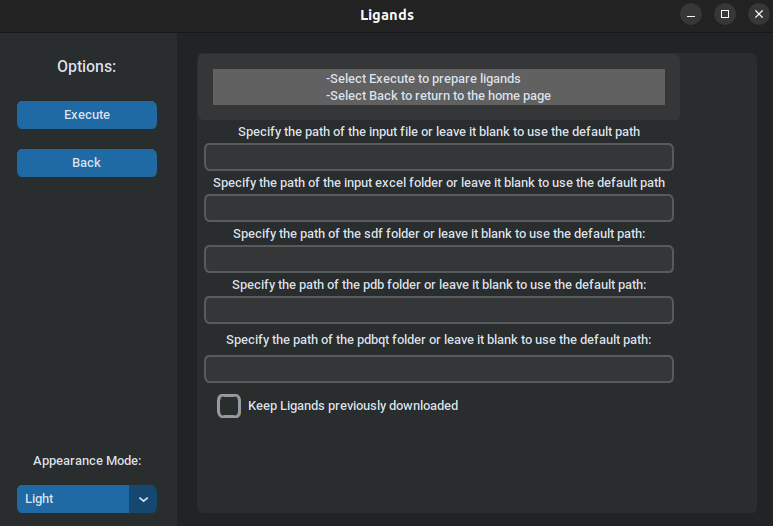
\includegraphics[scale=0.6]{immagini/ligands.png}
    \caption{Sezione \textbf{Ligands} della GUI}
    \label{fig:ligands}
\end{figure}

\begin{figure}[H]
    \centering
    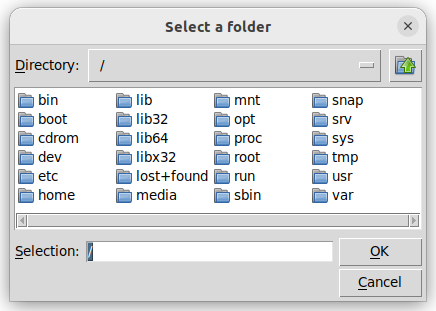
\includegraphics{immagini/browseFoldersLigands.png}
    \caption{\textbf{Browse folders}}
    \label{fig:browse folders ligands}
\end{figure}

La GUI per la preparazione dei ligandi richiama lo script \textbf{prepare\_ligands.py} discusso nella precedente sezioni, adattando l'interfaccia grafica ad esso senza eliminare alcuna funzionalità precedentemente illustrata per la versione da riga di comando e rispettando i dettami dell'\textbf{OOP}.\newline
Durante l'esecuzione viene mostrato un \textbf{pannello} (\ref{fig:ligands Execute}) in cui vengono descritte: le operazioni che si stanno effettuando, eventuali errori ed avvisi per l'utente, in modo tale che sia restituito un feedback all'utente relativo al progresso della preparazione dei ligandi. Al completamento di ogni fase sarà restituito un messaggio di avviso (figura: \ref{fig:progress completed ligands}) ed in caso di input non valido sarà restituito un messaggio di errore (figura: \ref{fig:Invalid input ligands}).

\begin{figure}[H]
    \centering
    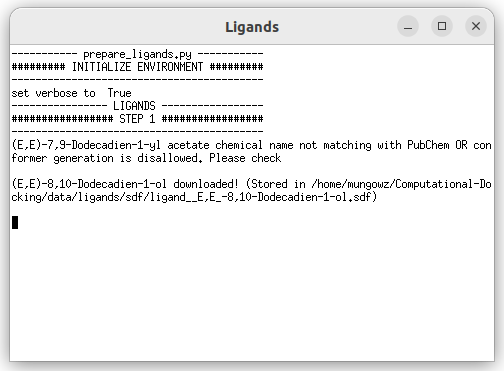
\includegraphics[scale=0.8]{immagini/ligandsExecute.png}
    \caption{\textbf{Pannello} dell'esecuzione dei ligandi}
    \label{fig:ligands Execute}
\end{figure}

\begin{figure}[H]
    \centering
    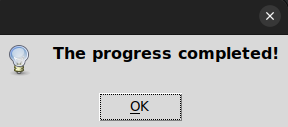
\includegraphics{immagini/progressCompletedLigands.png}
    \caption{Messaggio processo completato con successo}
    \label{fig:progress completed ligands}
\end{figure}

\begin{figure}[H]
    \centering
    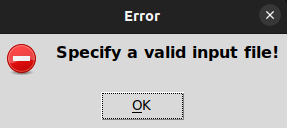
\includegraphics{immagini/invalidInputLigands.png}
    \caption{Messaggio di errore}
    \label{fig:Invalid input ligands}
\end{figure}

\subsection{Preparazione dei recettori tramite script} \label{Preparazione dei recettori script}
Lo script python \textbf{prepare\_receptors.py}, che esegue tale fase, viene eseguito da terminale mediante il comando:

\begin{lstlisting}[language=Python, label=lst:code11, caption={funzione prepare\_receptors}]
python prepare_receptors.py
\end{lstlisting}

Questo script può ricevere diversi argomenti in input:

\begin{itemize}
    \item $[-v] | [--verbose]$: serve per attivare il verbose e se non viene specificata tale opzione viene lasciata di default inattivo
    \item $[-E] | [--excel-folder]$: specifica la directory dei file \textit{.xlsx} di output, se non viene specificata tale opzione verrà scelta la directory di default
    \item $[-P] | [--pdb-folder]$: specifica la directory dei file \textit{.pdb} di output, se non viene specificata tale opzione verrà scelta la directory di default
    \item $[-p] | [--pdbqt-folder]$: specifica la directory dei file \textit{.pdbqt} di output, se non viene specificata tale opzione verrà scelta la directory di default
    \item $[-k] | [--keep-pdb-files]$: specificando questa opzione viene scelto di non cancellare i file delle proteine precedentemente scaricati, se non viene specificata tale opzione i file verranno cancellati
    \item $[-m] | [--margin]$: specificando questa opzione viene fornita in input la dimensione in \textit{angstrom} del margine della \textit{grid box} per le proteine se non viene specificata tale opzione viene impostato il valore di default ovvero 3
    \item $[-h] | [--help]$: stampa la spiegazione degli input per lo script.
\end{itemize}

Lo script quando eseguito andrà ad inizializzare i vari percorsi, e nel caso siano stati inseriti in input verrà controllata l'esistenza e la validità degli stessi. Nel caso non siano presenti le directory contenenti i file \textit{.txt}, \textit{.pdb} e .\textit{pdbqt}, queste verranno create automaticamente dall'applicazione a meno di input inseriti dall'utente e saranno cancellati i file precedentemente scaricati a meno di input contrario.\newline
Lo script richiama la funzione \textbf{selectReceptors} la quale si occupa di scaricare da \textbf{Pubchem} i file \textit{.pdb} corrispondenti alle proteine scelte. La funzione prende in input: 

\begin{itemize}
    \item \textit{pdb\_folder}, il path della directory di output per i file \textit{.pdb}
    \item \textit{excel\_folder}, il path della directory di output per i file \textit{.xlsx}
    \item \textit{verbose}, il flag relativo al verbose.
\end{itemize}

In output ci vengono dati i file \textit{.pdb} corrispondenti ai recettori scelti in input e un file \textit{.xlsx} contenente i risultati dell'operazione di download nominato \textit{info\_proteins.xls}.

\begin{lstlisting}[language=Python, label=lst:code12, caption={funzione selectReceptors}]
selectReceptors(pdb_folder, excel_folder, verbose)
\end{lstlisting}

All'interno di questa \textbf{selectReceptors} viene richiamata la funzione \textbf{RestApiSelection} la quale prende in input l'\textit{URL} di \href{https://www.rcsb.org/search}{PubChem}:

\begin{lstlisting}[language=Python, label=lst:code13, caption={funzione RestApiSelection}]
RestApiSelection(URL)
\end{lstlisting}

Questa funzione apre una \textbf{web view} sul sito di \href{https://www.rcsb.org/search}{PubChem} come mostrato nella figura \ref{fig:queryRecettori}, l'utente potrà digitare la propria query e scaricare i composti scelti selezionando il tasto in alto \textbf{Get Query}.\newline
La \textbf{web view} restituisce l'\textbf{URL} della pagina del database contenente i composti selezionati dalla query, il \textit{JSON} di tale pagina viene estratto e convertito nella struttura dati \textit{dizionario} di python tramite la funzione \textbf{loads} della libreria \textbf{json}.

\begin{lstlisting}[language=Python, label=lst:code14, caption={funzione json.loads}]
dictionary = json.loads(data)
\end{lstlisting}

Nel \textit{dizionario} restituito dalla funzione sarà contenuto l'elenco dei composti selezionati tramite la query.\newline
Il software rieseguirà direttamente la query tramite la funzione \textbf{get} contenuta nella libreria \textbf{requests}. Questa funzione permette di inviare una richiesta di tipo \textit{HTTP/1.1} prendendo in input \textbf{URL} della query al quale viene aggiunto l'elenco di composti da scegliere in formato \textit{JSON}, ciò eseguito convertendo il \textit{dizionario} precedentemente ottenuto in \textbf{JSON}
mediante la funzione \textbf{dump} della libreria \textbf{json}:

\begin{lstlisting}[language=Python, label=lst:code15, caption={funzione json.dump}]
dictionary = json.dump(dictionary)
\end{lstlisting}

La funzione \textbf{get} restituisce la lista di proteine da scaricare:

\begin{lstlisting}[language=Python, label=lst:code16, caption={funzione requests.get}]
requests.get(f"https://search.rcsb.org/rcsbsearch/v2/query?json={dictionary}")
\end{lstlisting}

La funzione \textbf{selectReceptors} richiama successivamente la funzione \textbf{downloadPdbs} che prende in input:

\begin{itemize}
    \item \textit{pdb\_list}, la lista di proteine precedentemente ottenuta
    \item \textit{outputh\_path}, il path della directory di output per i file \textit{.pdb}
    \item \textit{verbose}, il flag relativo al verbose.
\end{itemize}

La funzione ritorna in output i file \textit{.pdb} delle proteine contenute nella lista in input:

\begin{lstlisting}[language=Python, label=lst:code17, caption={funzione downloadPdbs}]
downloadPdbs(pdbs_list, output_path, verbose)
\end{lstlisting}

La funzione \textbf{downloadPdbs} richiama la funzione \textbf{fetchPDB} del pacchetto \textbf{ProDy}, questa prende in input:

\begin{itemize}
    \item \textit{protein\_code}, la proteina da scaricare
    \item \textit{folder}, il path della directory di output per i file \textit{.pdb}, nel nostro caso sarà impostato ad \textit{out\_path}
    \item \textit{compressed}, il flag per decidere se il file scaricato dovrà essere compresso oppure no, nel nostro caso il flag sarà impostato a \textit{False} per indicare che i file scaricati debbano essere già decompressi.
\end{itemize}

Tramite tale istruzione è possibile interfacciarsi con \textbf{PubChem} e scaricare di un singolo file \textit{.pdb} mediante richiesta \textit{FTP}, il download di tutte le proteine della lista avviene ciclando su tutti gli elementi di essa:

\begin{lstlisting}[language=Python, label=lst:code18, caption={funzione fetchPDB}]
fetchPDB(protein_code, folder=output_path, compressed=False)
\end{lstlisting}

Dopo aver effettuato il download di tutte i file \textit{.pdb} le informazioni relative al download ed ai file scaricati vengono salvati in un file \textit{.xlsx} chiamato \textit{info\_proteins.xlsx} che viene salvato nella directory \textit{/output/}.\newline
Lo script \textbf{prepare\_receptors.py} una volta terminata la funzione \textbf{selectReceptors} richiama \textbf{splitRepeatedResidues} che prende in input:

\begin{itemize}
    \item \textit{pdb\_folder}, il path della directory di output per i file \textit{.pdb}
    \item \textit{verbose}, il flag relativo al verbose.
\end{itemize}

Questa funzione si occupa di rimuovere i residui ripetuti memorizzati nel file \textit{.pdb} sotto la dicitura \textit{alternative location} o \textit{alt\_loc}:

\begin{lstlisting}[language=Python, label=lst:code19, caption={funzione splitRepeatedResidues}]
splitRepeatedResidues(pdb_folder, verbose, output_folder=None)    
\end{lstlisting}

Per accedere agli attributi dei file \textit{.pdb} utilizziamo la funzione \textbf{read\_pdb} del pacchetto \textbf{PandasPdb}, questa prende in input il nome del file \textit{.pdb}:

\begin{lstlisting}[language=Python, label=lst:code20, caption={funzione PandasPdb.read\_pdb}]
PandasPdb.read_pdb(pdb_file)
\end{lstlisting}

In particolare gli attributi \textit{A} e \textit{B} sono quelli ripetuti e i \textit{B} saranno quelli eliminati nella colonna \textit{alt\_loc}.\newline
Successivamente viene richiamata dallo script la funzione \textbf{deleteHeteroatomsChains}, la quale prende in input:

\begin{itemize}
    \item \textit{pdb\_folder}, il path della directory di output per i file \textit{.pdb}
    \item \textit{verbose}, il flag relativo al verbose.
\end{itemize}

Questa funzione si occupa di rimuovere le catene di eteroatomi contenute nel file \textit{.pdb}, queste sono evidenziate nel file tramite un loro attributo ovvero la keyword \textit{HETATM}, una volta rimosse, le catene vengono salvate. 

\begin{lstlisting}[language=Python, label=lst:code21, caption={funzione deleteHeteroatomsChains}]
deleteHeteroatomsChains(pdb_folder, verbose)
\end{lstlisting}

L'estrazione degli attributi dai file \textit{.pdb} avviene anche in questo caso tramite la funzione \textbf{read\_pdb} precedentemente descritta.\newline
Lo script \textbf{prepare\_receptors.py} richiama successivamente la funzione \textbf{splitChains} che prende in input: 

\begin{itemize}
    \item \textit{pdb\_folder}, il path della directory di output per i file \textit{.pdb}
    \item \textit{verbose}, il flag relativo al verbose.
\end{itemize}

Questa funzione si occupa di dividere le catene di residui che formano la struttura della proteina mantenendo soltanto le catene distinte, cioè quelle catene che hanno solo una sequenza aminoacidica distinta e non ripetuta da altre catene. 

\begin{lstlisting}[language=Python, label=lst:code22, caption={funzione splitChains}]
splitChains(pdb_folder, verbose)    
\end{lstlisting}

Tramite la funzione \textbf{parsePDB} della libreria \textbf{prody} viene ricostruita la struttura proteica attraverso oggetti come: la lista delle molecole, la lista degli atomi e dei residui, questa viene rappresentata da un oggetto della classe \textbf{AtomGroup} restituito dalla funzione \textbf{parsePDB}.

\begin{lstlisting}[language=Python, label=lst:code23, caption={funzione parsePDB}]
atoms = parsePDB(protein_file)
\end{lstlisting}

La ricostruzione della struttura proteica avviene tramite la vista gerarchica della struttura, ciò viene implementata tramite il metodo \textbf{getHierView} della classe \textbf{AtomGroup}:

\begin{lstlisting}[language=Python, label=lst:code24, caption={atoms.getHierVieW}]
atoms.getHierVieW()
\end{lstlisting}

Vengono quindi esaminate tutte le sequenze, sempre tramite la funzione \textbf{parsePDB}, e scelte solo le sequenze distinte, infine vengono salvate in un file tutte le catene distinte come se fossero delle proteine attraverso la funzione \textbf{writePDB} di \textbf{prody}, questa funzione prende in input:

\begin{itemize}
    \item \textit{filename}, il nome del file
    \item \textit{new\_atoms}, il composto da salvare
\end{itemize}

Questi file prenderanno il nome della proteina principale al quale viene aggiunto un underscore (\textit{\_}) seguito dal nome della catena distinta salvata nel file.

\begin{lstlisting}[language=Python, label=lst:code25, caption={writePDB}]
writePDB(filename, new_atoms)
\end{lstlisting}

Lo step successivo nella preparazione dei recettori è effettuato dalla funzione \textbf{prepareReceptors}, che prende in input:

\begin{itemize}
    \item \textit{pdb\_folder}, la directory con i file \textit{.pdb} in input
    \item \textit{pdbqt\_folder}, la directory con i file \textit{.pdbqt} in output
    \item \textit{verbose}, il flag relativo al verbose
    \item \textit{charges\_to\_add}, la carica da aggiungere alle proteine.
\end{itemize}

La funzione restituisce la conversione in file \textit{.pdbqt} dei corrispondenti i file \textit{.pdb} dati in input.

\begin{lstlisting}[language=Python, label=lst:code26, caption={prepareReceptors}]
prepareReceptors(pdb_folder, pdbqt_folder, verbose)
\end{lstlisting}

La funzione \textbf{prepareReceptors} utilizza lo script \textbf{prepare\_receptors4} offerto dalla suite \textbf{ADFR}. In realtà viene utilizzata una versione modificata di tale script: \textbf{replacePrepareReceptor4.sh}. Questa versione modificata tramite bash scripting sostituisce la carica di Gasteiger con la carica in input ovvero \textit{charges\_to\_add} che nel nostro caso sono cariche di Kollman come specificate dalla stringa \textit{"Kollman"}. Tramite questo script si effettua la corretta conversione da \textit{.pdb} a \textit{.pdbqt}. Lo script viene richiamato tramite riga di comando dalla funzione mediante il comando \textbf{prepare\_receptor}:

\begin{lstlisting}[language=bash, label=lst:code27, caption={comando per convertire file da \textit{.pdb} a \textit{.pdbqt}}]
prepare_receptor -r pdb_file_path -A checkhydrogens -C charges_to_add -e -o pdbqt_folder
\end{lstlisting}

Nell'istruzione sopra:

\begin{itemize}
    \item \textit{pdb\_file\_path} indica la directory con i file \textit{.pdb} in input ed è specificata tramite lo switch \textit{-r}
    \item \textit{checkydrogens} indica l'opzione tramite la quale vengono controllati gli atomi di idrogeno specificata lo switch \textit{-A}    
    \item \textit{charges\_to\_add} indica la carica usata in input impostata tramite lo switch \textit{-C} 
    \item \textit{pdbqt\_folder} indica la directory con i file \textit{.pdbqt} in output specificata tramite lo switch \textit{-o}
\end{itemize}

Tramite tale istruzione è possibile effettuare la conversione di un singolo file, mentre la conversione di tutti i \textit{.pdb} avviene ciclando su tutti i file nella directory corrispondente.\newline
L'ultima fase nella preparazione dei ligandi consiste nella creazione delle \textit{grid box}, mediante la funzione \textbf{createGridboxes} richiamata dallo script \textbf{prepare\_receptors.py}, la funzione prende in input:

\begin{itemize}
    \item \textbf{pdb\_folder}, la directory contenente i file \textit{.pdb} 
    \item \textbf{gridbox\_outputh\_folder}, la directory di output per le \textit{grid box}
    \item \textbf{margin}, la dimensione in \textit{angstrom} del margine della \textit{grid box}
    \item \textbf{verbose}, il flag relativo al verbose.
\end{itemize}

Per ogni proteina ottenuta deve essere creata una \textit{grid box}, questa definisce lo spazio conformazionale dove si colloca la proteina, è definita da:

\begin{itemize}
    \item Un centro
    \item Le dimensioni
    \item L'esaustività, la quale sarà utilizzata da qualsiasi software da \textbf{AutoDock Vina} per la ricerca delle pose possibili del ligando.
\end{itemize}

Una \textit{grid box} definisce la regione delle proteine dove il docking viene effettuato. Qualsiasi altra regione al di fuori dalla \textit{grid box} non verrà presa in considerazione durante il processo di docking.\newline
Le \textit{grid box} sono un input richiesto da \textbf{AutoDock Vina} ma non da altri software per il docking.\newline

\begin{lstlisting}[language=Python, label=lst:code28, caption={createGridboxes}]
createGridboxes(pdb_folder, gridbox_output_folder, margin, verbose)
\end{lstlisting}

Per ogni proteina vengono estratti gli attributi contenuti nel proprio file e viene richiamata da \textbf{createGridboxes} la funzione \textbf{createGridbox}, questa prende in input: 

\begin{itemize}    
    \item \textbf{ppdb}, l'insieme di attributi del file \textit{.pdb} ottenuti come oggetto della classe \textbf{AtomGroup} restituito dalla funzione \textbf{parsePDB}
    \item \textbf{protein\_path}, il file \textit{.pdb} corrispondente ad una singola proteina
    \item \textbf{gridbox\_outputh\_folder}, la directory di output per le \textit{grid box}
    \item \textbf{margin}, la dimensione in \textit{angstrom} del margine della \textit{grid box}
    \item \textbf{verbose}, il flag relativo al verbose.
\end{itemize}

La funzione \textbf{createGridbox} costruisce una \textit{grid box} per una singola proteina utilizzando gli attributi del file \textit{.pdb} rispettando i parametri precedentemente definiti per una \textit{grid box}.

\subsection{Preparazione dei recettori tramite GUI}
La preparazione dei recettori tramite GUI avviene selezionando il tasto \textbf{Receptors} nella sezione \textbf{Preparation} del software. All'interno della pagina relativa alla preparazione dei recettori premendo il tasto \textbf{Execute} è possibile effettuare i procedimenti precedentemente spiegati nella sezione relativa all'esecuzione tramite script (\ref{Preparazione dei recettori script}). Premendo il tasto \textbf{Back} è possibile tornare alla sezione \textbf{Preparation} relativa alla preparazione degli input.
Come si osserva nella figura \ref{fig:receptors} all'interno di tale sezione sono presenti delle \textbf{entry} dove è possibile specificare diversi input tra cui:

\begin{itemize}
    \item la directory dei file \textit{.xlsx} di output
    \item la directory dei file \textit{.pdb} di output
    \item la directory dei file \textit{.pdbqt} di output
    \item il valore del margine delle \textit{grid box}
\end{itemize}

Se lasciate vuote queste entry verrano impostate le configurazioni di default. E' presente anche un \textbf{checkbox} il quale se selezionato permette di mantenere i file precedentemente scaricati che altrimenti verrebbero cancellati.\newline
Per andare a selezionare direttamente nel file system del PC i file e le directory richieste sono stati implementati rispettivamente i tasti \textbf{Browse files} e \textbf{Browse folders}, come è visibile in figura \ref{fig:ligands}, \ref{fig:browse files receptors} e \ref{fig:browse folders receptors}.

\begin{figure}[H]
    \centering
    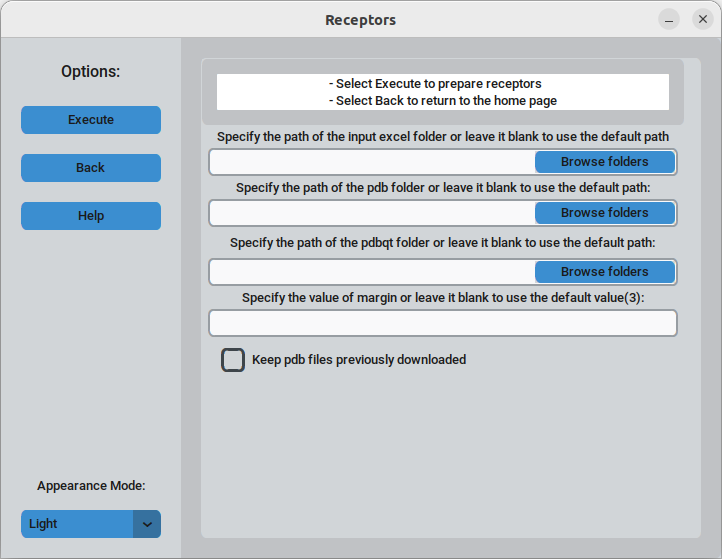
\includegraphics[scale=0.6]{immagini/receptors.png}
    \caption{Sezione \textbf{Receptors} della GUI}
    \label{fig:receptors}
\end{figure}

\begin{figure}[H]
    \centering
    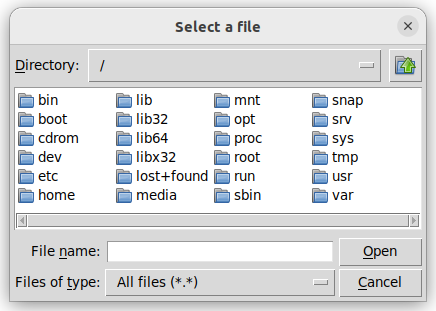
\includegraphics{immagini/browseFilesReceptors.png}
    \caption{\textbf{Browse files}}
    \label{fig:browse files receptors}
\end{figure}

\begin{figure}[H]
    \centering
    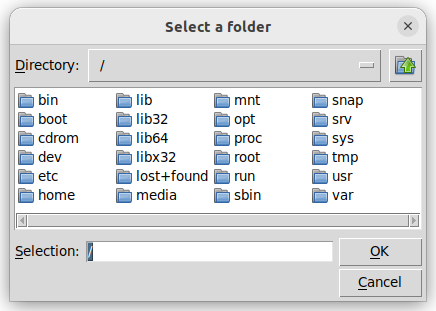
\includegraphics{immagini/browseFoldersReceptors.png}
    \caption{\textbf{Browse folders}}
    \label{fig:browse folders receptors}
\end{figure}

La GUI per la preparazione dei ligandi richiama lo script \textbf{prepare\_ligands.py} discusso nella precedente sezioni, adattando l'interfaccia grafica ad esso senza eliminare alcuna funzionalità precedentemente illustrata per la versione da riga di comando e rispettando i dettami dell'\textbf{OOP}.\newline
Durante l'esecuzione viene mostrato un \textbf{pannello} (\ref{fig:receptors execute}) in cui vengono descritte: le operazioni che si stanno effettuando, eventuali errori ed avvisi per l'utente, in modo tale che sia restituito un feedback all'utente relativo al progresso della preparazione dei ligandi. Al completamento di ogni fase sarà restituito un messaggio di avviso (figura: \ref{fig:progress completed proteins}) ed in caso di input non valido sarà restituito un messaggio di errore (figura: \ref{fig:Invalid input proteins}).

\begin{figure}[H]
    \centering
    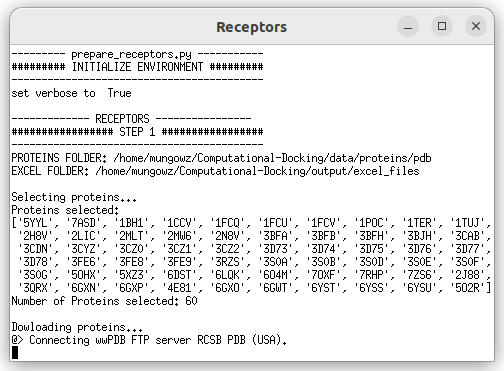
\includegraphics[scale=0.8]{immagini/receptorsExecution.png}
    \caption{\textbf{Pannello} dell'esecuzione dei recettori}
    \label{fig:receptors execute}
\end{figure}

\begin{figure}[H]
    \centering
    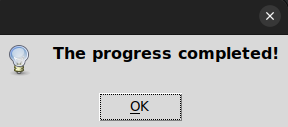
\includegraphics{immagini/progressCompletedReceptors.png}
    \caption{Messaggio processo completato con successo}
    \label{fig:progress completed proteins}
\end{figure}

\begin{figure}[H]
    \centering
    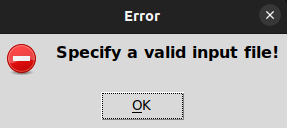
\includegraphics{immagini/invalidInputReceptors.png}
    \caption{Messaggio di errore}
    \label{fig:Invalid input proteins}
\end{figure}

\section{Docking tramite script}
Dopo aver ottenuto i ligandi ed i recettori può essere effettuato il \textbf{Docking}, questo avviene mediante lo script bash \textbf{performDocking.sh}, il comando per eseguire lo script è:

\begin{lstlisting}[language=bash, label=lst:code29, caption={Comando per eseguire performDocking}]
./performDocking.sh -s vina
\end{lstlisting}

Lo script quando viene lanciato prende in input il parametro opzionale $-h$, che mostra il prompt con le istruzioni per l'uso dello script.\newline
Lo script prende in input la cartella dove sono presenti:

\begin{itemize}
    \item Le proteine in formato \textit{.pdbqt}
    \item I ligandi in formato \textit{.pdbqt}
    \item Le gridbox in formato \textit{.txt}
\end{itemize}

Successivamente creerà la cartella \textit{/output/docking} dove verranno salvati i risultati del docking, per ogni coppia proteina-ligando verrà eseguito il seguente comando:

\begin{lstlisting}[language=bash, label=lst:code30, caption={Comando per eseguire il docking con Autodock Vina}]
vina --config gridbox_file.txt --receptor receptor_file.pdbqt --ligand ligand_file.pdbqt --out "{percorso_directory_software_installato}/output/docking/vina/cartella_nome_recettore/cartella_nome_ligando/out.pdbqt" --log "{percorso_directory_software_installato}/output/docking/vina/cartella_nome_recettore/cartella_nome_ligando/log.txt"
\end{lstlisting}

Nell'istruzione sopra:
\begin{itemize}
    \item \textit{Vina} è il commando per eseguire il docking con \textbf{AutoDock Vina}
    \item \textit{gridbox\_file.txt} è la gridbox in input relativa al recettore \textit{receptor\_file.pdbqt}, la gridbox è specificata dallo switch \textit{$--$config}
    \item \textit{receptor\_file.pdbqt} è il file di input del recettore nel formato \textit{.pdbqt}, specificato dallo switch \textit{$--$receptor}
    \item \textit{ligand\_file.pdbqt} è il file di input del ligando nel formato \textit{.pdbqt}, specificato dallo switch \textit{$--$ligand}
    \item \textit{directory di output}, specificata dallo switch \textit{$--$out}
    \item \textit{log di output}, specificato dallo switch \textit{$--$log}.
\end{itemize}

Questo comando è in grado di eseguire il docking per una sola coppia proteina-ligando, per effettuare il docking su tutte le coppie deve essere eseguito tale comando per tutte le proteine su ogni ligando. Tale istruzione creerà una cartella per ogni proteina il cui nome corrisponde a quello della proteina (\textit{cartella\_nome\_recettore}), all'interno di tale cartella verranno create tante cartelle quanti sono i ligandi con cui vengono studiate le pose, il nome delle sottocartelle è quello dei rispettivi ligandi (\textit{cartella\_nome\_ligando}). All'interno di ogni sottocartella sono contenuti due file:

\begin{itemize}
    \item Un file \textit{.pdbqt} nominato out.pdbqt, il corrispondente output per la coppia proteina-ligando
    \item Un file \textit{.txt} nominato \textit{log.txt}, contenente le informazioni relative alla posa ottenuta. 
\end{itemize}

Se si considera la proteina \textbf{1fcu} ed il ligando \textbf{bentazone} entrambi utilizzati nel caso di esempio, verrà creata una cartella nominata \textbf{1cfu} contenente una sottocartella nominata \textbf{bentazone} contenente a sua volta un file \textit{log.txt} e \textit{out.pdbqt}.

All'interno del file di log è possibile ricavare le seguenti informazioni:

\begin{itemize}
    \item \textit{mode}, il numero della posa calcolata in modo randomico
    \item \textit{affinity}, indica la stabilità del legame, misurata in kcal/mol, della coppia proteina-ligando ed è calcolata sul valore dell'energia di legame, più il valore è negativo o l'affinità di legame è bassa, più il ligando-recettore è stabile
    \item \textit{dist from best mode} indica la \textit{root-mean-square deviation (RMSD)} ossia la distanza media tra gli atomi, questo parametro si divide in due valori: \textit{lower bound (l. b)} distanza minima ed \textit{upper bound (u. p.)} distanza massima.
\end{itemize}

È possibile selezionare la migliore conformazione tra i risultati di \textbf{autoDock Vina}, ma non la migliore conformazione per una particolare proteina. Durante la ricerca delle pose il programma mantiene la conformazione data e inizia la selezione delle pose da lì. Per questo motivo si ottiene sempre un valore RMSD pari a 0. Di seguito il file di log del docking per la proteina \textbf{1fcu} combinata con il ligando \textbf{bentazone}:

\begin{figure}[H]
\begin{verbatim}
#################################################################
# If you used AutoDock Vina in your work, please cite:          #
#                                                               #
# O. Trott, A. J. Olson,                                        #
# AutoDock Vina: improving the speed and accuracy of docking    #
# with a new scoring function, efficient optimization and       #
# multithreading, Journal of Computational Chemistry 31 (2010)  #
# 455-461                                                       #
#                                                               #
# DOI 10.1002/jcc.21334                                         #
#                                                               #
# Please see http://vina.scripps.edu for more information.      #
#################################################################

WARNING: The search space volume > 27000 Angstrom^3 (See FAQ)
Detected 8 CPUs
Reading input ... done.
Setting up the scoring function ... done.
Analyzing the binding site ... done.
Using random seed: -2136627046
Performing search ... done.
Refining results ... done.

mode |   affinity | dist from best mode
     | (kcal/mol) | rmsd l.b.| rmsd u.b.
-----+------------+----------+----------
   1         -6.6      0.000      0.000
   2         -6.0      1.874      3.171
   3         -6.0     31.288     32.713
   4         -5.9     28.684     30.487
   5         -5.9     31.907     33.061
   6         -5.9     30.972     32.563
   7         -5.7      3.854      6.764
   8         -5.7      2.808      5.241
   9         -5.7     28.294     29.592
Writing output ... done.
\end{verbatim}
\caption{File di log del docking per la coppia proteina-ligando \textbf{1fcu-bentazone}}
\label{fig:file di log}
\end{figure}

\section{Docking tramite GUI}
Il docking tramite GUI avviene selezionando il tasto \textbf{Docking} nella sezione \textbf{Home page} del software. All'inteno della pagina relativa al docking premendo il tasto \textbf{Execute} è possibile effettuare il docking, premendo il tasto \textbf{Back} è possibile tornare alla sezione \textbf{Home Page}.
Come si osserva nella figura \ref{fig:docking} all'interno di tale sezione sono presenti delle \textbf{entry} dove è possibile specificare diversi input tra cui:

\begin{itemize}
    \item la directory dei file \textit{.pdbqt} delle proteine di input
    \item la directory dei file \textit{.pdbqt} dei ligandi di input
    \item la directory dei file \textit{.txt} delle gridbox di input
    \item la directory dei log e dell'output del docking
\end{itemize}

Se lasciate vuote queste entry verrano impostate le configurazioni di default. E' presente anche un \textbf{checkbox} il quale se selezionato permette di mantenere i file precedentemente scaricati che altrimenti verrebbero cancellati.\newline
Per andare a selezionare direttamente nel file system del PC i file e le directory richieste sono stati implementati rispettivamente i tasti \textbf{Browse files} e \textbf{Browse folders}, come è visibile in figura \ref{fig:docking} e \ref{fig:browse folder docking}.

\begin{figure}[H]
    \centering
    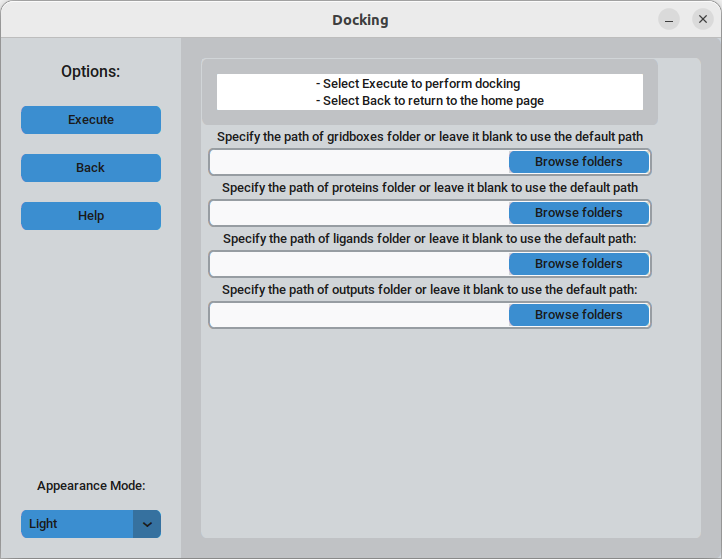
\includegraphics[scale=0.6]{immagini/docking.png}
    \caption{Sezione \textbf{Receptors} della GUI}
    \label{fig:docking}
\end{figure}

\begin{figure}[H]
    \centering
    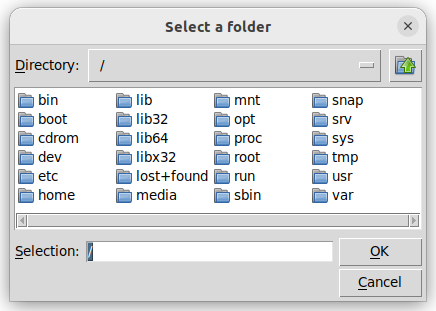
\includegraphics{immagini/browseFoldersDocking.png}
    \caption{\textbf{Browse files}}
    \label{fig:browse folder docking}
\end{figure}

La GUI per il \textbf{docking} richiama lo script \textbf{performDocking.sh} discusso nella precedente sezioni, adattando l'interfaccia grafica ad esso senza eliminare alcuna funzionalità precedentemente illustrata per la versione da riga di comando e rispettando i dettami dell'\textbf{OOP}.\newline
Durante l'esecuzione viene mostrato un \textbf{pannello} (\ref{fig:docking execution}) in cui vengono descritte: le operazioni che si stanno effettuando, eventuali errori ed avvisi per l'utente, in modo tale che sia restituito un feedback all'utente relativo al progresso della preparazione dei ligandi. Al completamento di ogni fase sarà restituito un messaggio di avviso (figura: \ref{fig:progress completed docking}) ed in caso di input non valido sarà restituito un messaggio di errore (figura: \ref{fig:Invalid input docking}).

\begin{figure}[H]
    \centering
    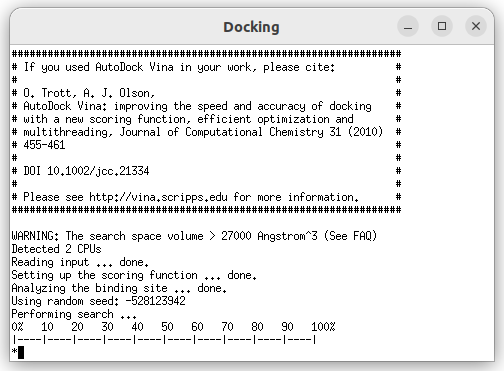
\includegraphics[scale=0.8]{immagini/dockingExecute.png}
    \caption{\textbf{Pannello} dell'esecuzione del \textbf{docking}}
    \label{fig:docking execution}
\end{figure}

\begin{figure}[H]
    \centering
    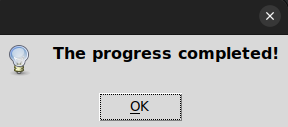
\includegraphics{immagini/progressCompletedDocking.png}
    \caption{Messaggio processo completato con successo}
    \label{fig:progress completed docking}
\end{figure}

\begin{figure}[H]
    \centering
    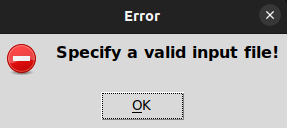
\includegraphics{immagini/invalidInputDocking.png}
    \caption{Messaggio di errore}
    \label{fig:Invalid input docking}
\end{figure}